\chapter{Beispiele}

\section{Namen}

prof: \prof\\
proff: \proff\\
chu: \chu\\
chuf: \chuf\\
rli: \rli\\
rlif: \rlif\\
fsc: \fsc\\
fscf: \fscf

\section{Todos}

\xxx
\xxx[foobar]

\section{Syntax Highlighting}

Benötigt Python und pygments. Lässt sich mittels \mintinline{console}{$ pip install pygments} installieren. 

Und noch ein Block Beispiel:

\begin{src}{console}
$ grunt test:e2e # Unit Tests ausführen
\end{src}

und in \cref{lst:hello-world} eines fürs Programmcodeverzeichnis:

\begin{srclst}[label=lst:hello-world]{python}{Hello World beispiel}
	print 'hello world'
\end{srclst}

\section{Pseudocode}
Siehe \cref{alg:test-pseudocode}, wenn auch in dieser Arbeit wohl nicht nötig.

\begin{pseudocode}[label=alg:test-pseudocode]{Irgendwas}
	\State $foo \gets 42$
	\Comment{bar?}
	\While{$foo > 0$}
	\State $foo\gets a-1$
	\State $foo$ ausgeben
	\EndWhile
\end{pseudocode}


\section{User stories}


\begin{scrumepic}[label=epic:example]{Example epic}
	Als XY, will ich die XY können, sodass ich XY kann.
	\storyacceptance	
	Gegeben
	\storyitem{XY,}
	\storyitem{einen modernen Webbrowser (Internet Explorer 10 oder neuer und alle Evergreen\footnote{Browser die sich automatisch auf dem neusten Stand halten} Browser),}
	wenn XY, dann soll XY.
\end{scrumepic}

\begin{scrumstory}[label=story:example]{Example story}
	Als XY, will ich die XY können, sodass ich XY kann.
	\storyacceptance	
	Gegeben
	\storyitem{XY,}
	\storyitem{YZ},
	wenn XY, dann soll XY.
\end{scrumstory}


In \cref{epic:example} \dots


\section{Wichtige Entscheidungen}
\begin{decision}{Frontend Framework}
	Im Kontext der Evaluation eines für die Aufgabenstellung passenden Frontend JavaScript Frameworks wurde, um eine rapide Entwicklung mit geringen Support-Risiken zu erreichen für XY und gegen X, Y, Z und andere entschieden und wir akzeptieren, dass der Einsatz mit gewissen Einarbeitungsaufwänden verbunden ist.
\end{decision}


\section{Tabelle}

tabularx \& booktabs

Shortcut mit mytable

% \mytable{cols}{content}{caption}{label without tab:}
\mytable{ll}{
Col1 & Col2\\
\midrule
Row1 & Row1\\
Row2 & Row2\\
}{Example table}{example-table}

In \cref{tab:example-table} ist \dots


\section{Referenzieren}

Mit cref, für weit entfernte Referenzen vref

vref: In \vref{tab:example-table} ist \dots


\section{Glossar}
Siehe \path{glossary_acronyms.tex}. Habe einige Beispiele, die wir evtl. ohnehin verwenden werden beibehalten.

\gls{ba} \\
\acs{avt}\\
\acf{avt} \\\
\dots

\section{Subfigure}

\begin{figure}[H]
	\centering
	\begin{subfigure}{0.49\textwidth}
		\centering
		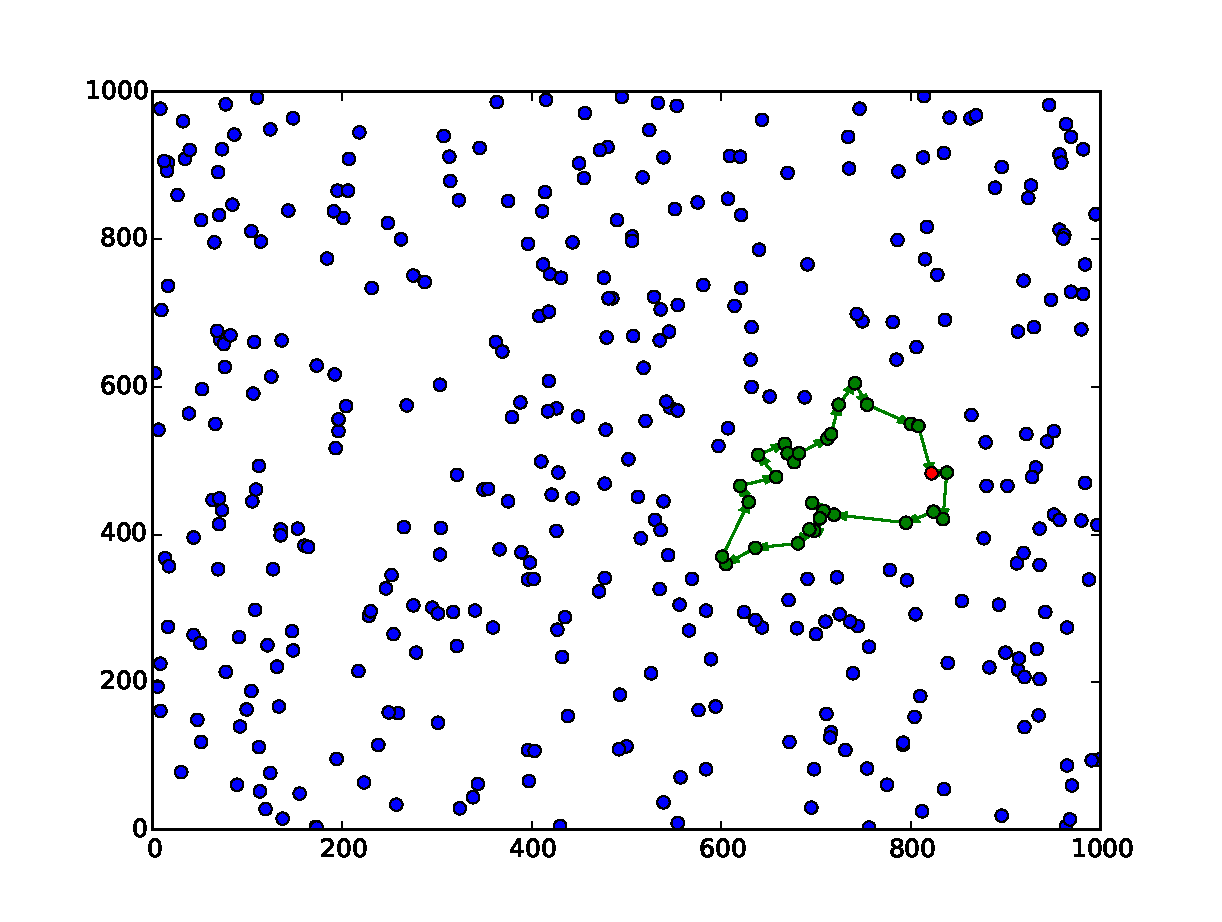
\includegraphics[width=\linewidth,trim=1cm 1cm 1cm 1cm,clip]{fig/genalg-proto-tsp}
		\caption{Von A nach A}
		\label{fig:genalg-proto-tsp}
	\end{subfigure}
	\begin{subfigure}{0.49\textwidth}
		\centering
		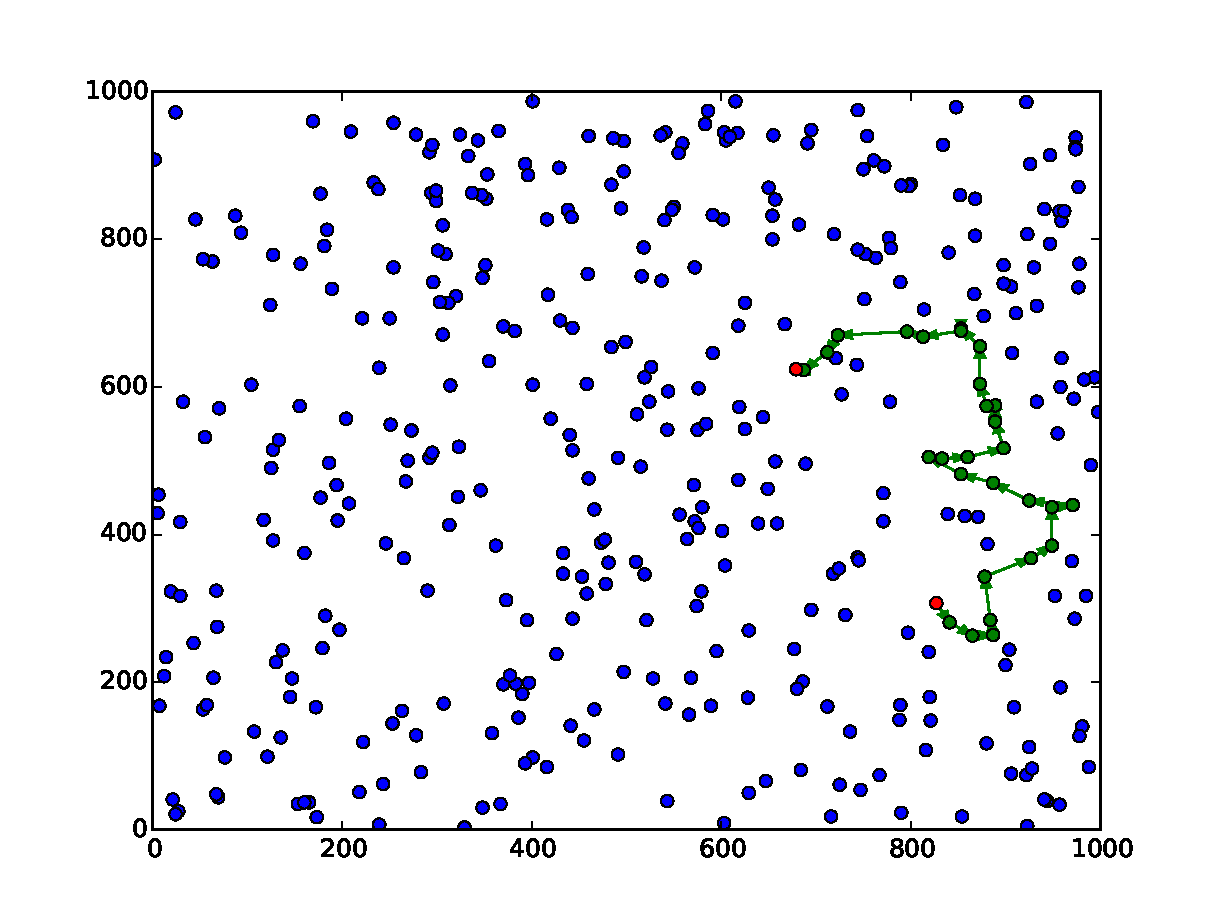
\includegraphics[width=\linewidth,trim=1cm 1cm 1cm 1cm,clip]{fig/genalg-proto-route}
		\caption{Von A nach B}
		\label{fig:genalg-proto-route}
	\end{subfigure}
	\caption{Prototyp des Genetischen Algorithmus}
	\label{fig:genalg-proto}
\end{figure}

\section{Other Packages}
Siehe \path{style.sty}, vermutlich schon etwas dabei. Die Reihenfolge der Imports ist teilweise relevant.